\chapter{Подавление артефактов, вызванных наличием сильнопоглощающих включений} \label{chapt2}


В данной главе рассматривается задача исправления ошибок реконструкции, возникающих при томографии сложных объектов, содержащих области сильного поглощения рентгеновского излучения.
Так как наличие подобных артефактов (рис. \ref{im:high_absorb_artifacts}) сильно затрудняет последующий анализ результатов томографии, необходимо использовать алгоритмы, учитывающие специфику исследуемого объекта и позволяющие уменьшить влияние сильнопоглощающих (или металлических) включений в объект.
Обычно для подавления этих артефактов на алгоритмическом уровне используют методы, основанные на предобработке синограммы, модификации алгебраических методов на основе методов максимального правдоподобия или выпуклого программирования.
В данной главе предлагается метод, использующий специально построенную модель формирования артефактов, позволяющий уменьшить влияние таких включения на восстановленную картину.
Предложенная модель может быть выражена в виде ограничений-неравенств, которые, будучи добавлены к целевой задаче оптимизации алебраического метода, составляют задачу квадратичного программирования и позволяют использовать математический аппарат методов численной условной оптимизации.

\begin{figure}
\centering
\begin{tabular}{@{}c@{}c}
  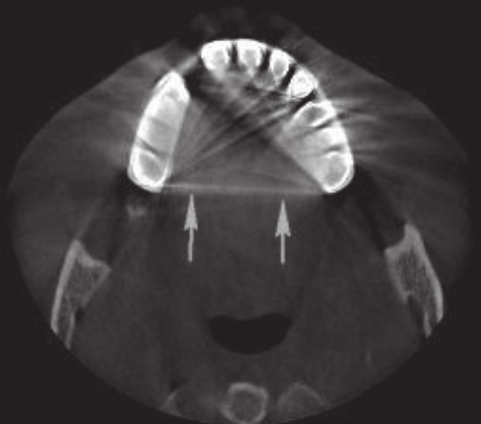
\includegraphics[width=0.3\textwidth]{part2_img/tooth_artifacts_med}
  &
  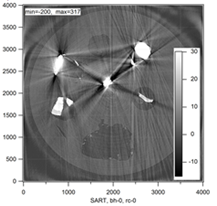
\includegraphics[width=0.3\textwidth]{../Presentation/images/high_absorb_artifacts}
\\
\end{tabular}
\caption{Примеры артефактов, вызванных наличием сильнопоглощающих включений в объекте}
\label{im:high_absorb_artifacts}
\end{figure}

Основной вклад данной главы состоит в следующем: предлагается модель формирования артефактов, вызванных наличиием сильнопоглощающих включений, предлагается метод восстановления на основе данной модели, исследуются результаты работы данного метода на различных входных данных, а также производится сравнение результатов восстановления методов, основанных на квадратичном программировании и на использовании ``мягких'' аддитивных квадратичных штрафов. 
Все предложенные алгоритмы в главе сопровождаются вычислительным экспериментом, результаты которых анализируются в соответствующем разделе.

\section{Модель возникновения артефактов}
\label{sect_2_0}

Основное предположение, лежащее в основе предлагаемой модели, состоит в том, что причиной возникновения артефактов является неправильная интерпретация измеренных данных, и в результате непраивльно постренная оптимизационная функция.
Проходя через металлическое включение, лучи рентгеновского излучения поглощаются сильнее чем в остальных учатсках объекта.
В результате в пиксели детектора, в которые попадают эти лучи, попадает излучение интенсивностью меньше или сравнимой с уровенем шума.
В результате либо получится слишком зашумленное измерение, соотношение сигнал-шум которого неприемлемо для восстановления, либо после прохождения АЦП в измерениях с этих лучей будет записано значение 0.
Однако все что можно сказать про эти измерения, это что реальное значение в них лежит где-то в интервале $[0, \delta_{min})$, где $\delta_{min}$ --- минимальный порог срабатывания детектора, или уровень шума.
Поэтому и восстановление измерений для этих лучей неоходимо производить с учетом их значений как неравенств.

Предлагаемая модель может быть выражена в оптимизационной задаче алгебраического метода в виде ограничений-неравенств.
Обозначим за $\delta_{min}$ порог активации пикселя (или уровень шума).
После обычной для томографии процедуры логарифмирования условие для пикселей $j$ в которых интенсивность пришедшего излучения меньше порога ($I_j < \delta_{min}$) можно записать условие $P_j > \ln\frac{I_0}{\delta_{min}} = \delta$.
Учитывая, что в терминах алгебраического метода $P_j = \sum_i f_i w_{ij}$, оптимизационная задача с учетом предложенной модели будет выглядеть следующим образом:

\begin{equation}
  \label{eq:quadprog_ineq}
  \begin{cases}
  \Norm{P^{\textup{изм.}} - W(f)} \rightarrow \min\limits_f & w.r.t \\
  \sum_i f_{i} w_{ij} > \delta, & \mbox{если } P^{\textup{изм.}}_j = \delta \\
  f_{i} \geq 0
  \end{cases}
\end{equation}

В условия-неравенства оптимизационной задачи (\ref{eq:quadprog_ineq}) так же введены условия-ограничения на неотрицательность значений логарифма линейной функции плотности поглощения рентгеновского излучения $f_i$.
Так как функционал ошибки квадратичный, а ограничения - линейные, для решения этой минимизационной задачи эффективным будет применить метод квадратичного программирования.
При этом в формулировке оптимизационной задачи присутствует полная матрица преобразования Хафа $w_{ij}$.
Как и в случае с алгебраическим методом, решение задачи возможно при использовании итеративной градиентной минимизации, ввиду ее огромной размерности.
Действительно, количество элементов матрицы приблизительно составляет $\sqrt{2} * n * n_\varphi \times n * n$ для изображения размером $n \times n$ и $n_\varphi$ проекционных углов.
При этом ненулевые значения для каждого столбца находятся только в $\approx n$ ячейках, делая возможным использование инструментария для работы с разреженными матрициы.
Несмотря на это, при $n = 256, n_\varphi = 180$ и использовании чисел с плавающей точкой двойной точности (тип данных float64) и способа хранения разреженных матриц ``compressed sparse row'' такая матрица в оперативной памяти вычислителя будет занимать порядка 170Мб.
При этом для традиционных методы решения задачи QP требует рассчета гессиана матрицы целевой функции, то есть матрицы $W W^{\mathrm{T}}$, которая в разреженном виде занимает 11Гб в оперативной памяти и ее невозможно обрабатывать стандартными реализациями ПО для режения задач выпуклого и квадратичного программирования.
Поэтому необходима разработка специальной процедуры, не требующей работы с такой огромной матрицей в явном виде, а лишь с результатами ее умножения на вектор, которые могут быть выражены в виде преобразований обработки изображений

Дальнейшая структура главы следующая: сначала на изображениях малого разрмера будет показана применимость подхода, основанного на предложенной модели возникновения артефактов; после этого будут предложены два подхода к переносу результатов на изображения большего размера, и будет произведено сравнение этих подходов на модельном примере.

\section{Задача квадратичного программирования малой размерности}
\label{sect_2_1}

Для оценки применимости подхода, использующего условную оптимизацию для подавления металлических артефактов, рассматривается модельное распределение линейного коэффициента поглощения размера 10х10 пикселей, содержащее два объекта существенно разной поглощающей способности (рис. \ref{fig:qp_phantom_10by10} а).
Первый объект --- высокопоглощающая (металлическая) ``скобка'' слева фантома, второй --- ``крест'' из более прозрачного материала.
Ожидается что наличие металлического закрывающего объекта затруднит восстановление внутреннего мелкого объекта.
Синограмма данного фантома представлена на рис. \ref{fig:qp_phantom_10by10} б).

\begin{figure}
    \centering
    \begin{tabular}{@{}c@{}c}
    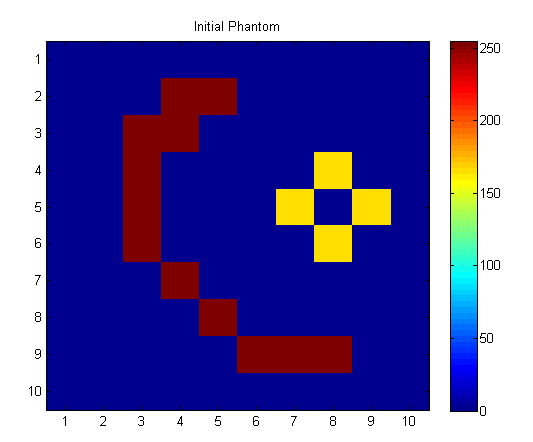
\includegraphics[width=0.4\textwidth]{../Presentation/images/qp_phantom} 
    &
    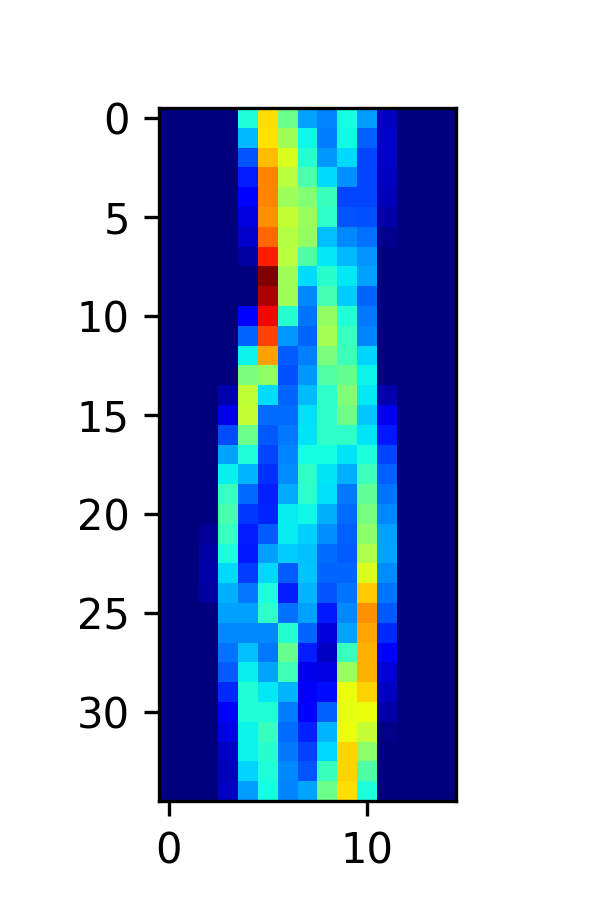
\includegraphics[width=0.4\textwidth]{../Presentation/images/qp_sino} 
    \\
    а) & б)
    \end{tabular}
    \caption{а) Модельный фантом размера 10х10 пикселей. б) синограмма}
    \label{fig:qp_phantom_10by10}
\end{figure}

Порог $\delta$ для экспериментов подбирался таким образом, чтобы обрезать максимумы синограммы.
Значение порога было 800, размер пикселя был 1х1.
Значение сильнопоглощающего включение было 250, слабопоглощающего обхекта - 160.
При расчете синограммы использовалось 35 проецкионых углов, равномерно распределенных в интервале от 0 до 180 градусов.

Для вычисления синограммы используется стандартная процедура прямой томографической проекции.
Однако для формирования входных данных для решения задачи квадратичного программирования необходимо вычислить матрицу проекции $W$ поэлементно.

\section{Вычисление значений элементов матрицы проекции}

Действие оператора томографической поекции $W$ на дискретное изображение распределение линейного коэффициента поглощения $f$ легко вычисляется в виде алгоритма обработки изображений.
Более подробное описание этого приведено в предыдущей главе.
В этом параграфе  предстоит совершить ``обратное'' --- имея возможность делать прямую проекцию вычислить значения элементов матрицы $w_{ij}$
В данном разделе будет построен алгоритм вычисления элементов матрицы, используя декомпозицию оператора $W$ по отдельным лучам проекции а так же линейность самого преобразования томографической проекции.

Действие оператора проекции на изображение обозначается как $\mathbf{p} = W\mathbf{f}$.
Введем калибровочные изображения $\mathbf{f}^{(k)} = \delta_{ik}$, имеющие только один ненулевой пиксель.
За $\delta_{ik}$ обозначен символ Кронекера, т.е. тензор, значения которого удовлетворяют $\delta_{ik} = 1 \text{, если} i = j \text{, иначе} 0$.
Любое изображение на входе оператора проекции можно представить в виде линейной комбинации калиборочных: $\mathbf{f} = \sum_k f_k \mathbf{f}^{(k)}$.
Значит для вычисления элементов линейного оператора $W$ можно затабулировать результаты его применения ко всем калибровочным изображениям:

\begin{equation}
  \label{eq:w_on_calib_img}
  p_j = \left(W \mathbf{f}^{(k)} \right)_j = \sum_i w_{ij} \delta_{ik} = w_{kj}
\end{equation}

В результате алгоритм вычисления значений матрицы $W$ представлен на алг. \ref{alg:hough_matrix}:

\begin{algorithm}[H]
 \KwData{линейный размер входного изображения $n$, количество углов проекции $n_\varphi$}
 \KwResult{значения элементов матрицы $w_{ij}$}
 инициализация нулями матрицы (возможно, разреженной) $W \in \textbf{Mat}\left(nn, nn_\varphi)\right)$\;
 \For{каждого пикселя $k = 0 \dots nn$}{
  вычислить значение проекции калибровочного изображения $\mathbf{p}^{(k)} = W \mathbf{f}^{(k)}$\;
  обновить значение жлементов $w_{kj}$ используя формулу (\ref{eq:w_on_calib_img})\;
 }
 \caption{Алогритм вычисления элементов матрицы $w_{ij}$}
 \label{alg:hough_matrix}
\end{algorithm}

\section{Метод восстановления}

Формулировка задачи оптимизации, решение которой приводит к восстановленному изображению, приведена в (\ref{eq:quadprog_ineq}).
Это задача квадратичного программирования, хорошо известная и имеющая много готовых реализаций решающего ПО в популярных математических пакетах.
Для проверки подхода были использованы реализации пакета quadprog на языке Matlab \cite{coleman1996reflective} и пакета cvxopt для языка Python \cite{andersen2013cvxopt}.
Опишем в общем случае алгоритм решения задачи квадратичного программирования.

В общем случае задача квадратичного программирования формулируется как 

\begin{equation}
  \label{eq:quadprog_general}
  \begin{cases}
  \frac 1 2 x^\mathrm{T}Px + q^\mathrm{T}x \rightarrow \min\limits_x & w.r.t \\
  Gx \preceq h \\
  Ax = b\,
  \end{cases}
\end{equation}

где $P$ --- симметричная положительно определнная матрица, а $Gx \preceq h$ означает поэлементное выполнение неравенства.
Одним из эффективных подходов к решению оптимизации такого вида являются методы внутренней точки.
На протяжении всей оптимизационной процедуры решение находится внутри области, удовлетворящей ограничениям.
Постепенно с приближением к оптимуму, решению позвояют приближаться ближе и ближе к границе, и ,в конце концов, удовлетворяет необходимой точности решения задачи.
Это достигается за счет введения так называемых барьерных функций для ограничений-неравенств, вклад котрых ослабляется с ходом оптимизации.
А именно, для каждого неравенства $g_i^\mathrm{T}x \leq 0$ вводится аддитивный член в целевую функцию вида $\phi_i(x) = -\frac 1 t \log{\left(- g_i^\mathrm{T}x \right)}$.
Эти функции являются гладкими аппроксимациями индикаторной функции ограничений $I_i(x) = 0 \text{, если } g_i^\mathrm{T}x < 0 \text{, иначе} +\inf$.
Легко получается выражение для первой и второй производной барьерной функции:

\begin{equation} 
\label{eq:barrier_grads}
\begin{split}
\nabla \phi_i(x) &= \frac 1 t \frac {g_i}{-g_i^\mathrm{T}x} \\
\nabla^2 \phi_i(x) &= \frac 1 t \frac {g_i g_i^\mathrm{T}} {\left( g_i^\mathrm{T}x \right)^2}
\end{split}
\end{equation}

Задача (\ref{eq:quadprog_general}) принимает вид

\begin{equation}
  \label{eq:quadprog_barrier}
  \begin{cases}
  \frac 1 2 x^\mathrm{T}Px + q^\mathrm{T}x + \frac 1 t \phi(x) \rightarrow \min\limits_x & w.r.t \\
  Ax = b\,
  \end{cases}
\end{equation}

где $\phi(x) = \sum_i \phi_i (x) = \sum_i {-\log{\left(- g_i^\mathrm{T}x \right)}}$ --- полная функция со всеми барьерными штрафами. 
Такая задача оптимизации решается методом Ньютона, а именно с помощью итеративной минимизации вида
%\begin{equation} \notag
\begin{gather}
\left(
  \begin{matrix}
  P + \frac 1 t \nabla^2 \phi_i(x) & A ^\mathrm{T} \\
  A & 0
  \end{matrix}
  \right)
  \left(
  \begin{matrix}
  \Delta x \\ \nu
  \end{matrix}
  \right)
  =
  \left(
  \begin{matrix}
  -x^\mathrm{T}P - q^\mathrm{T} - \frac 1 t \nabla \phi(x) \\ 0
  \end{matrix}
  \right),
\end{gather}
где за $\Delta x$ обозначен очередной инкремент итерации.
Далее метод барьерных функций представляет собой последовательное решение ``центрирующих'' задач вида (\ref{eq:quadprog_barrier}) для растущей последовательности параметров $t, \mu t, \mu^2 t \dots$

Метод барьерных функций представляет собой общий инструментарий для рещения задач выпуклого программирования. 
В контексте сформулированной в (\ref{eq:quadprog_ineq}) оптимизационной задачи получается ... \todo{вывести значения P, A G для томографической задачи}


%\end{equation}


\section{Результаты восстановления}

\begin{comment}

\section{Описание образца} \label{sect_2_1_1}
\begin{figure}
  \centering
  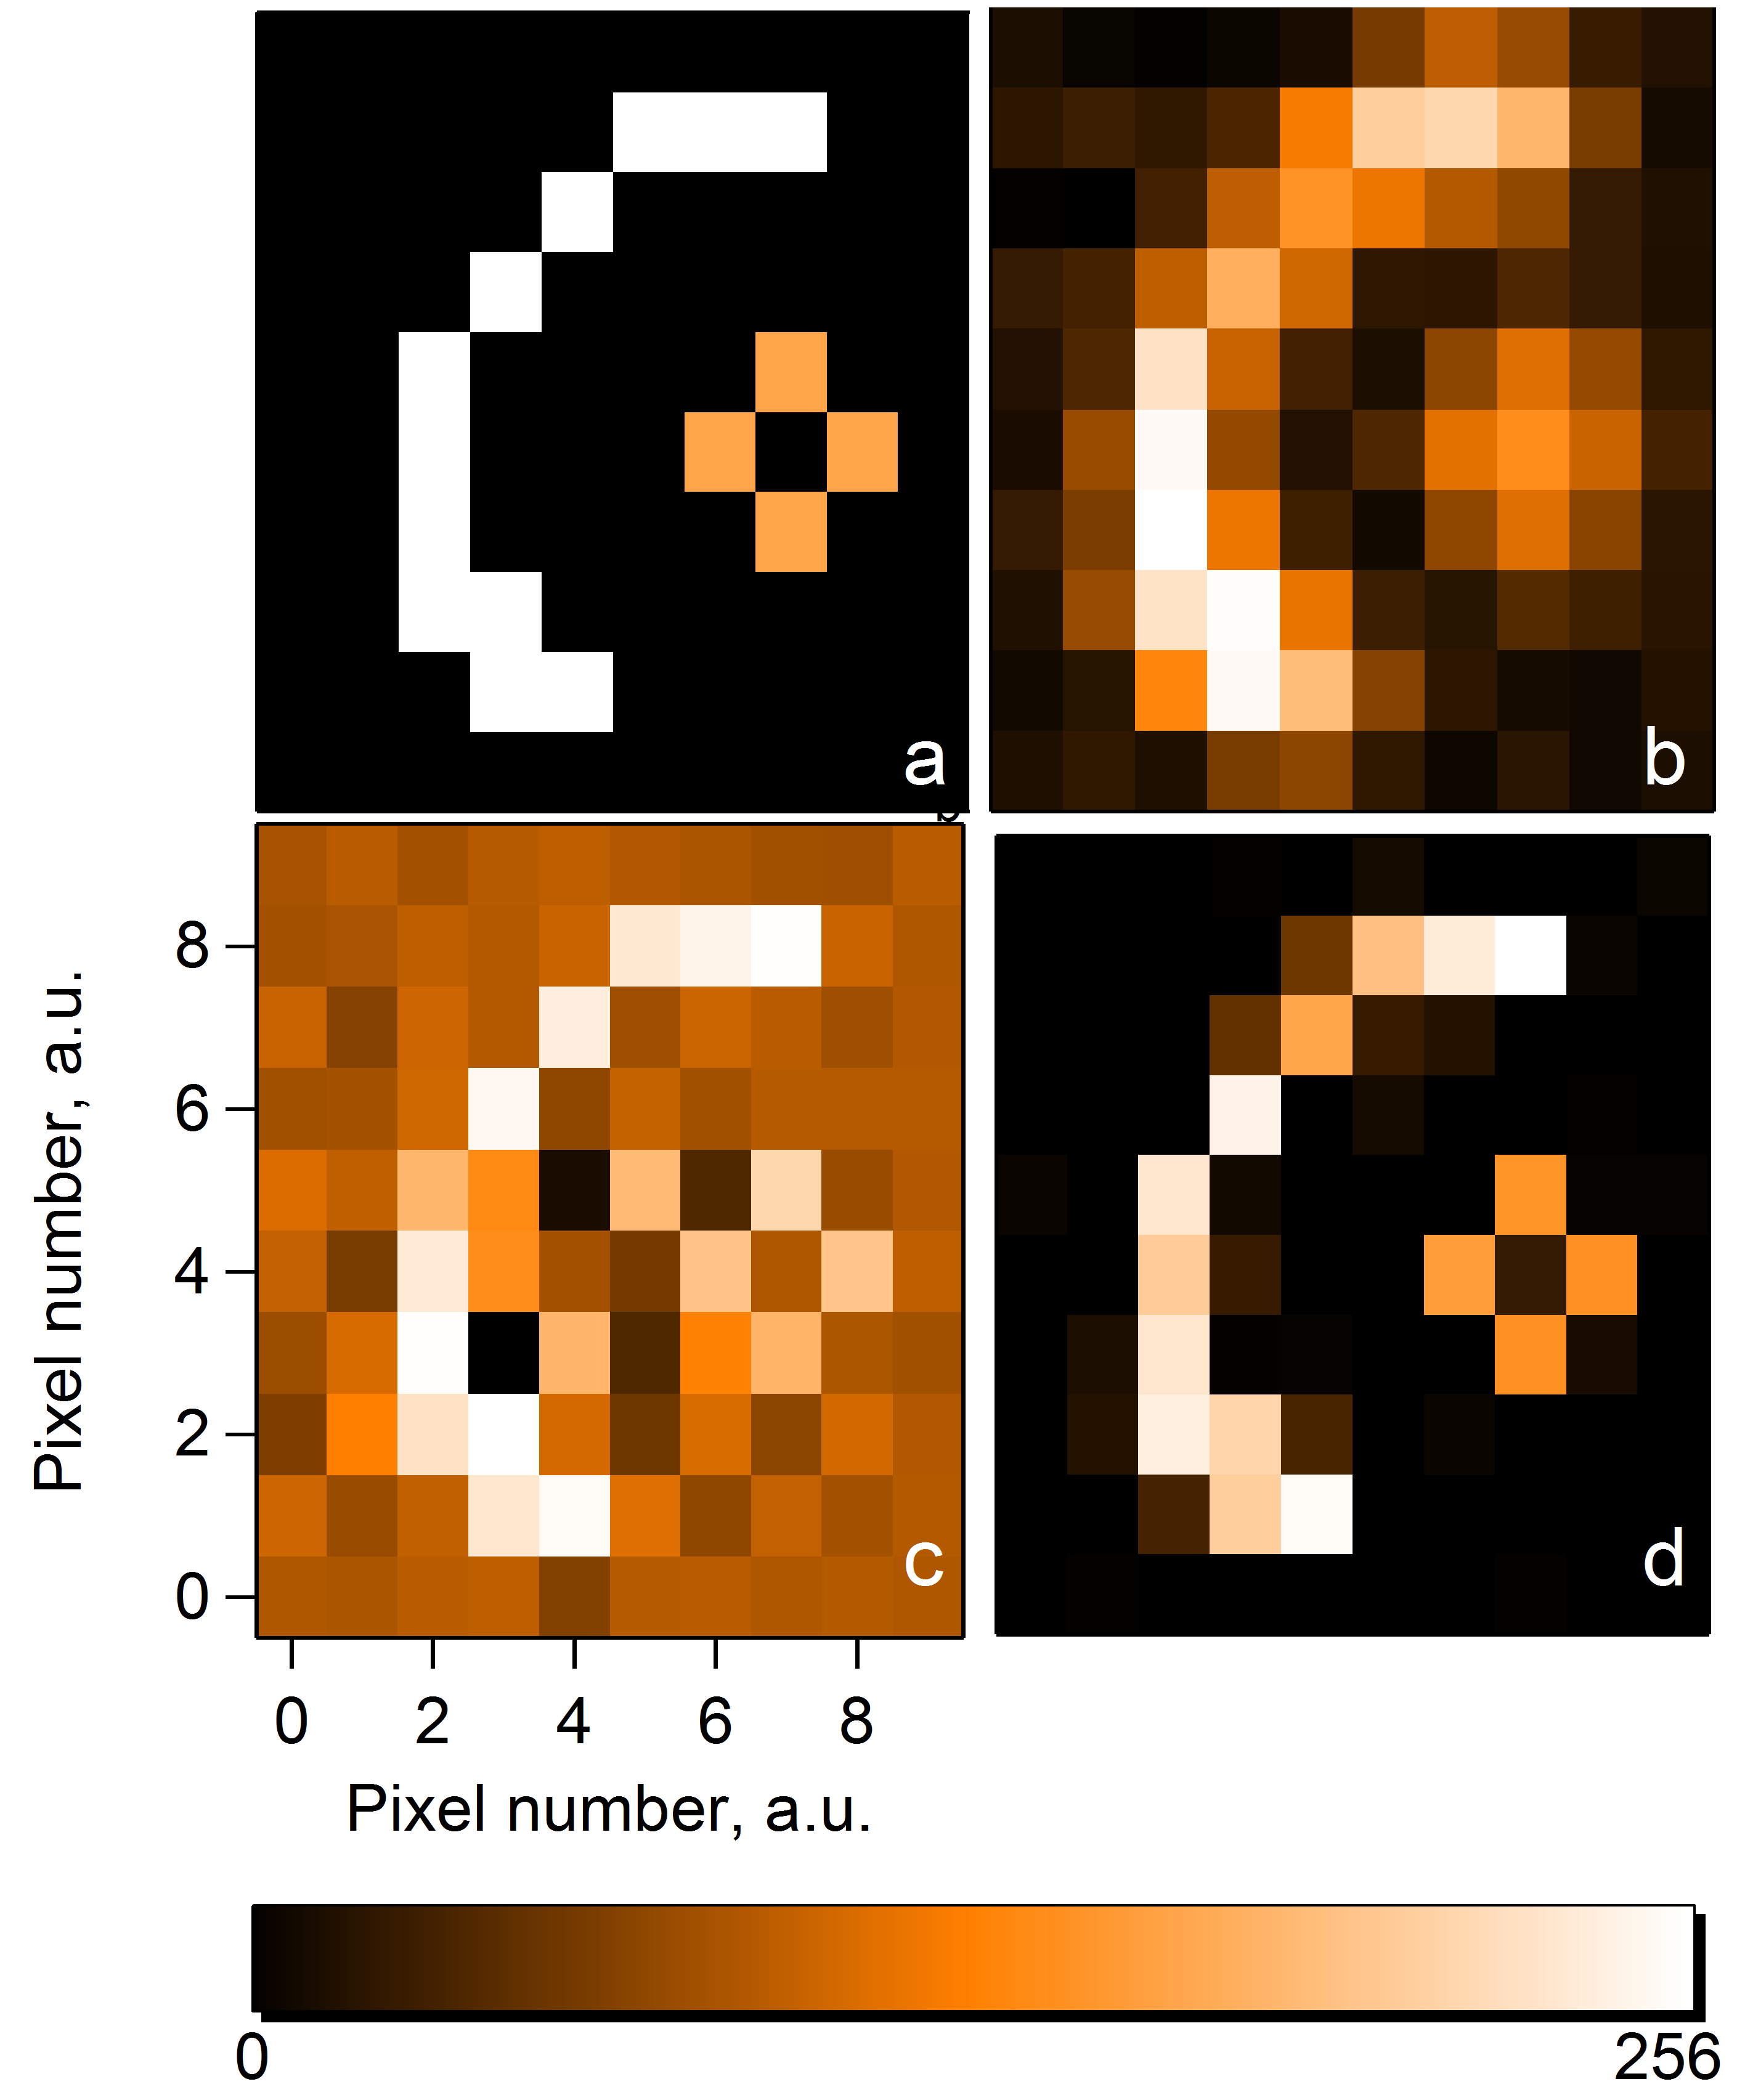
\includegraphics[width=0.7\textwidth]{part2_img/quadprog}
  \caption{Слева сверху - фантом использовавшийся для симуляций. Справа сверху - результат восстановления FBP. Слева снизу - результат восстановления квадратичным программированием без ограничений-неравенств. Справа снизу - результат восстановление квадратичным программированием с ограничениями-неравенствами (предложенный метод)}
  \label{im:quadprog}
\end{figure}

Для симуляции использовался фантом, изображенный на рисунке \ref{im:quadprog}a).
Это распределение вещества в сечении 10х10 пикселей, состоящее из двух объектов: скобки с высоким коэффициентом поглощения и крестика с нормальным уровнем поглощения.
Сгенерированная синограмма обрезалась по заданному значению порога, эмитируя эффект металлических включений.
Таким образом, была расчитана матрица проекции $\omega$, такая, что проеция $P = \omega \mu$ происходила по закону:

\begin{equation}
\label{eq:quadprog_projection}
P_j = 
\begin{cases}
\sum_i \mu_{i}\omega_{ij} , & \mbox{если} \mu_{i}\omega_{ij} < \mbox{порог} \\
\mbox{порог}, & \mbox{иначе}
\end{cases}
\end{equation}

, где $i$ - номер пикселя распределения, $j$ - номер луче проекции, порог подбирался таким образом, чтобы обрезать максимумы синограммы.
Значение порога было = 800, размер пикселя был 1х1.
Значение сильнопоглощающего включение было 256.
При расчете синограммы использовалось 35 проецкионых углов, равномерно распределенных в интервале от 0 до 180 градусов.

\todo{вставить синограмму}

На рисунке \ref{im:quadprog}b представлено восстановление полученной синограммы методом свертки и обратной проекции. 
Целью данного подраздела является улучшение данного восстановения методом квадратичного программирования.

Задача квадратичного программирования для воссатновления компьютерной томографии может быть сформулирована как 

\begin{equation}
  \label{eq:quadprog_eq}
  \begin{cases}
  \Norm{P^{\textup{изм.}} - P(\mu)} \rightarrow \min_{\mu} & w.r.t \\
  \sum_i \mu_{i} \omega_{ij} = P_j, & j = 1 \dots 35
  \end{cases}
\end{equation}

То есть условная минимизация с ограничениями типа равенства.
Результаты восстановления с помощью решения задачи (\ref{eq:quadprog_eq}) представлены на рисунке \ref{im:quadprog}с.

Следующим шагом в развитии этого метода восстановления является учет ограничений типа неравенства (\ref{eq:quadprog_projection}), учитывающих эффект сильного поглощения металлов.
задача (\ref{eq:quadprog_eq}) переходит в следующую:
\begin{equation}
  \label{eq:quadprog_ineq}
  \begin{cases}
  \Norm{P^{\textup{изм.}} - P(\mu)} \rightarrow \min_{\mu} & w.r.t \\
  \sum_i \mu_{i} \omega_{ij} = P_j, & \mbox{если} P^{\textup{изм.}}_j < \mbox{порог} \\
  \sum_i \mu_{i} \omega_{ij} > \mbox{порог}, & \mbox{если} P^{\textup{изм.}}_j = \mbox{порог}
  \end{cases}
\end{equation}

Восстановление с помощью решения (\ref{eq:quadprog_ineq}) изображено на рисунке \ref{im:quadprog}d.
Для восстановления использовался метод \cite{quadprog_algo}.
Как видно из рисунка, квадратичное программирование с условиями неравенствами обеспечивает лучшее восстановление границ и интенсивностей исходного фантома. 
Значения интенсивностей на разных частях восстановленых фантомов приведены в таблице \ref{tb:quadprog_res}:

\begin{table}[h]
\label{tb:quadprog_res}
\centering
\begin{tabular}{ r| c| c| c| c|}
 & \ref{im:quadprog}a & \ref{im:quadprog}b & \ref{im:quadprog}c & \ref{im:quadprog}d \\ \hline
скобка & $255 \pm 0$ & $146 \pm 25$ & $233 \pm 30$ & $225 \pm 26$ \\ \hline
крест & $164 \pm 0$ & $69 \pm 3.6$ & $170 \pm 19.5$ & $151 \pm 5.2$ \\ \hline
\end{tabular}
\caption{Средние значения и стандартное отклонение интенсивностей в разных областях исследуемого фантома}
\end{table}

Так же можно заметить, что использование квадратичного программирование с ограничениями типа неравенство обеспечивет лучшие значения интенсивностей с меньшим значением отклонения.

\end{comment}

\section{Результаты} \label{sect_2_1_2}

\todo{текст ECMS\_2015}

\section{Мягкие ограничения на неравенства} \label{sect_2_2}

In this paper, we improve the results achieved in \cite{chukalinaway}. First, we provide a robust to noise and admissible to efficient optimization methods way to express the inequalities introduced in \cite{chukalinaway}. Second, we evaluate the method's performance on a simulated phantom data. The phantom data was simulated to remind a teeth with a metal object. And finally we evaluate the gain we get using the information in the inequalities against not using it at all.

The sections are organized as follows. Section \ref{s-approach} outlines the detail our approach to solve the problem. In Section \ref{s-phantom} the simulated phantom is presented. The obtained results are discussed in Section \ref{s-results}. Section \ref{s-conclusion} then concludes the whole paper.

% \section{Описание подхода}
\label{s-approach}
Let us denote the distribution of the attenuation coefficient in the reconstructed volume with $x \in \mathbb{R}^m$. The $p \in \mathbb{R}^n$ denotes the projection data detected during a scan. According to Beer-Lambert law the energy, detected at the detector cell, corresponding to $i$-th ray is expressed by the formula $p_i = I_0 * \exp(-a_i^T x)$, where $I_0$ is the source intensity, and $a_i$ is the row of the projection matrix $A$ corresponding to the $i$-th ray. A standard approach to find $x$ from the projection data is to take a logarithm and solve the linear system of equations: $Ax = r$, where
$r_i = \log(I_0) - \log(p_i)$. A standard way to get robust to noise reconstruction here is to use linear least squares:
\begin{equation} \label{eq:lls}
  \Norm{Ax - r}^2 \to \min\limits_{x}.
\end{equation}

Metal streak artifacts are caused mainly by photon starvation and noise. Mathematically it corresponds to the rays where $p_i$ is small or even zero. In latter case the logarithm is not defined and the simples way is just to ignore those rays solving instead of \eqref{eq:lls}:
\begin{equation}
  \label{eq:mask-lls}
  \Norm{P(Ax - r)}^2 \to \min\limits_{x},
\end{equation}
where matrix $P$ takes only those coordinates of a vector, at which $p_i \neq 0$. More precisely,
$$
P_{i,j} = \begin{cases}
  1, \quad\text{if $i = j$ and $p_i > 0$} \\
  0, \quad\text{otherwise}
  \end{cases}.
$$

It was suggested in \cite{chukalinaway} that even such problematic rays provide us with some information, namely that the weighted sum along such a ray has lower bound $a_i^T x > B$, for some suitable value of $B$ (for example, $B = \log I_0$), and we can use this information in a form of linear inequality constraints, solving the linear system with linear least squares approach:
\begin{equation}
  ||P(Ax - r)||^2 \to \min\limits_x, \quad\textrm{s.t. }  QAx \ge B,
\end{equation}
where $Q$ takes only those coordinates of a vector at which $p_i = 0$, opposite to the matrix $P$. Basically, $Q = E - P$, where $E$ is identity matrix.

This constraints being mathematically correct, are tight and are not robust against the noise in the projection data. Instead of tight constraints we propuse to use a soft version provided with a quadratic penalty method \cite{nocedal2006numerical} instead:
\begin{equation}
  \label{eq:soft-ineq}
  ||P(Ax - r)||^2 + \alpha ||[QAx - B]^-||^2 \to \min\limits_x,
\end{equation}
where $[y]^- = \min\{0, y\}$.

This functional provides a soft way to enforce the inequalities on the variables, but also allows to handle noise effects more smoothly. We can regulate the effect of that smoothing by manipulating $\alpha$: the greater $\alpha$ is tighter the effect of inequalities is.

The objective function \eqref{eq:soft-ineq} is convex and differentiable. We can effectively minimize it with Conjugate Gratient method (we used the implementation of this method, provided by the Python package \cite{scipy}). To speed-up computation of forward and backward tomographic projection operators we used ASTRA Toolbox \cite{palenstijn2011performance, van2015astra} which performs efficient evaluation of such operators on GPU.
\begin{figure}[h]
  \centering
  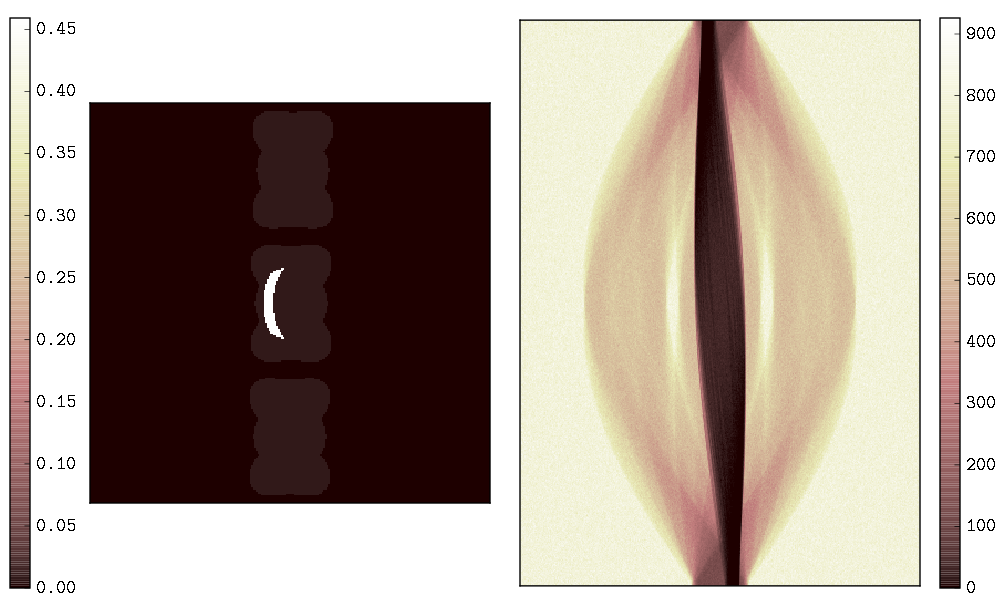
\includegraphics[scale=0.45]{part2_img/phantom-and-projection}
  \caption{The phantom (left) and its projection at $I_0 = 10^3$ photons (right).}
  \label{phantom-and-projection}
\end{figure}

\section{Описание образца}
\label{s-phantom}
To simulate the sinogram in $55$keV monochromatic mode we used a phantom imitating three teeth. Middle tooth contains titanium include imitating an implant (fig. \ref{phantom-and-projection}, left image). Pixel size is $0.005$cm. 2D field view size is $256 \times 256$ pixels. We used the XRayLib library \cite{brunetti2004library, schoonjans2011xraylib} to calculate the X-ray attenuation in each pixel for chosen energy. The sinogram (fig. \ref{phantom-and-projection}, right image) was calculated in a parallel scheme. We used $512$ rotation angles uniformly distributed in the interval $[0, \pi)$. The number of the detector cells is $362$, so that the diagonal of the phantom is projected on the detector without loosing any information. Such geometry choice allowed us to ignore the uniqueness of the solution issues which are related to the null-space of the projection operator and are ususally dealt with some sort of regularization techniques.

\section{Результаты}
\label{s-results}
To study the proposed approach we generated projections for different source intensities and draw several samples of Poisson noise at each source intensity.

For each projection we reconstructed the volume using Missing Data Least Squares \eqref{eq:mask-lls} and proposed Soft Inequalities Least Squares \eqref{eq:soft-ineq} approaches. The value of $\alpha$ was chosen to be equal to $50$.. The reconstructed volume was then compared to the original phantom and Mean Square Error was compute for such a pair.

In the figure \ref{sample} we can see an example of such reconstructions. In absence of the information encoded in the inequalities the metal artifacts are presented and there is a strong shadow in the cental tooth, while in the left image, reconstructed with Soft Inequalities approach those artifacts are significantly reduced.
\begin{figure}
  \centering
  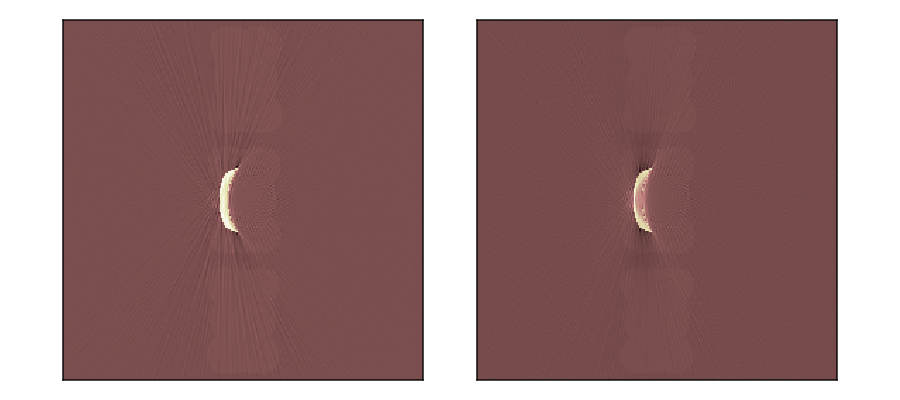
\includegraphics[scale=0.5]{part2_img/sample}
  \caption{Example of reconstruction with Soft Inequalities method (left)
    and Missing Data method (right).}
  \label{sample}
\end{figure}
In the figure \ref{error-plot} we can see the plot of MSE averaged over all the samples of noise for each noise level. The inequalities provide an improvement over ignoring such data at all noise levels.
\begin{figure}
  \centering
  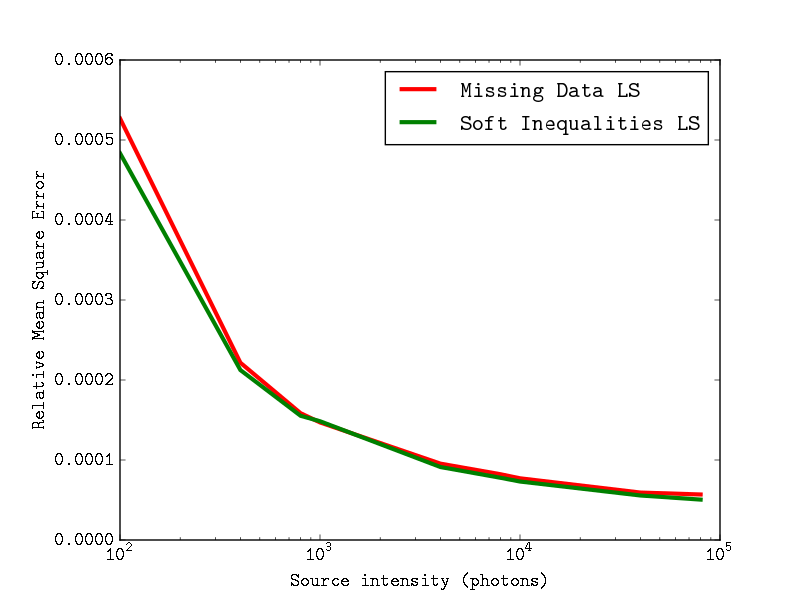
\includegraphics[scale=0.5]{part2_img/error-plot}
  \caption{The MSE value with respect to noise level.}
  \label{error-plot}
\end{figure}

\section{Выводы}
\label{s-conclusion}

Experiments shows that the information encoded in the inequalites, introduced in \cite{chukalinaway} carries a significant information which can be used to reduce metal-like artifacts in the reconstructions. We proposed a robust way to use this information in form of panaltized objective function. The proposed functional is suitable to be minimized with an efficient numerical algorithms enabling the approach to work on mid- and large-sized data. Proved to work, the method next should be deeper with respect to sensitivity to $\alpha$ and compared against the other approaches mentioned in the introduction. It is also seems possible to leave the penalty encoding the inequality constraints, replacing the least squares functional with more statistically suitable (for example, Poisson log-likelihood, used in MLEM) data fit functional.

\subsection{параметры моделирования и восстановления} \label{sect_2_3}
Параметры моделирования:
\begin{itemize}
  \item размером фантома (size, 65, 256),
  \item количеством углов проекции (n\_angles, 90, 512), 
  \item интенсивность пучка (i0, 1000)
  \item энергия пучка (45 кэв)
  \item форма фантома (три зуба и имплант-бумеранг)
  \item материалы фантома и импланта (Ca, Au)
  \item наличие импланта (в наличии)
  \item размер пикселя (0.05)
  \item наличием шума при прокеции, распределением шума (есть пуассоновский шум)
\end{itemize}

Параметры восстановления:
\begin{itemize}
  \item итераций 200 (где-то 300)
  \item $\alpha$ 30 и 300
\end{itemize}